%test results
\section{Experiment Results}
\label{section:results}

The proposed method has an exact way to identify whether a query audio clip has a matching registered song or not. Therefore this method can be considered as
a classifier. A classifier can be evaluated by the confusion matrix generated for a given sample. \ac{tp}, \ac{fp}, \ac{tn} and \ac{fn} were calculated
for each test case. Then accuracy and \ac{fp} rate was calculated for each test case. Reducing \ac{fp} rate is significant as much as increasing the accuracy
given that this method mainly focuses on identifying music on radio broadcasts. Accuracy and \ac{fp} rate can be calculated from the formulas given below. 

\begin{align*}
    \text{Accuracy} &= \frac{TP+TN}{TP+TN+FP+FN}\\
    \\
    \text{FP Rate} &= \frac{FP}{FP+TN}\\
\end{align*}

Keypoint ratio based threshold is proposed as the threshold measure in this method. Two experiments were done, one with keypoint count as threshold measure and the
other with keypoint ratio as threshold measure to validate the claim of keypoint ratio is better threshold measure. 

\subsection{Using Keypoint Count as Threshold}

Average accuracies for different threshold values are illustrated as shown in Figure \ref{fig:threshold_old} to identify the optimal threshold value to use. Since
the visualization clearly indicates a global peak value which is keypoint count of 69, that value can be used as the threshold value. This threshold value of 69 is
used in this experiment. 
\vspace{12pt}

Results of the experiment using keypoint count as the threshold measure are presented in Table \ref{tab:test_results_keypoint}. There is no clear
change between accuracies of pitch changes and tempo changes when using keypoint count as the threshold measure. Pitch changes and tempo changes
up to 20\% alteration can be identified with 92\%-98\% accuracy. 


\begin{figure}[H]
    \centering
    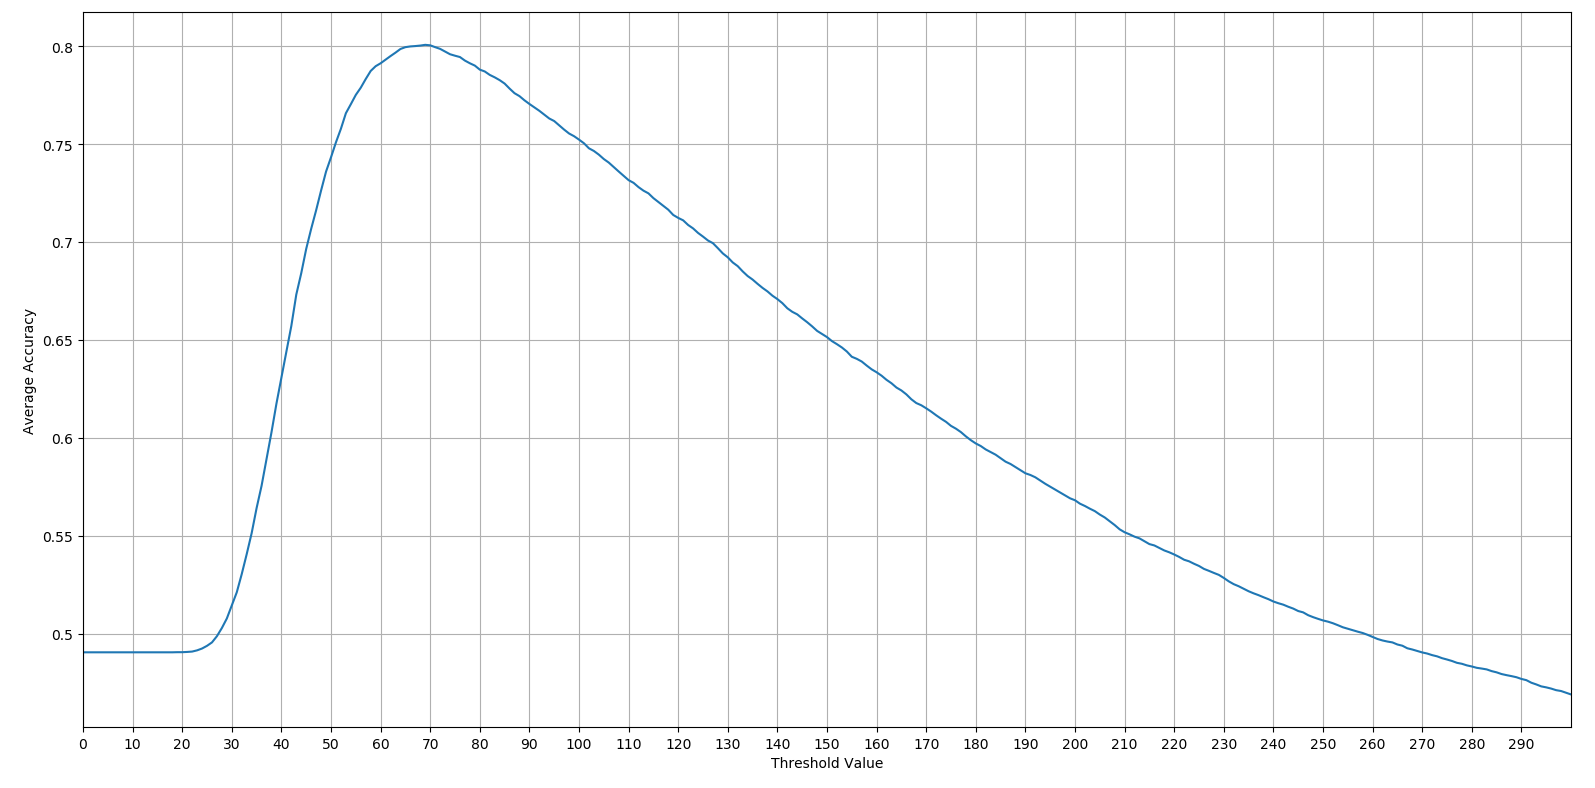
\includegraphics[scale=0.3]{threshold_adjusting_old.png}
    \caption{Average Accuracy Values for Different Threshold Values (Keypoint Count)}
    \label{fig:threshold_old}
  \end{figure}
  


\begin{table}[H]
    \begin{tabular}{|l|r|r|r|r|r|r|}
        \hline
        \textbf{Test Case}                  & \textbf{TP}   & \textbf{FP} & \textbf{TN} & \textbf{FN} & \textbf{Accuracy} & \textbf{FP Rate} \\ \hline
        Tempo Increase 10\%                & 509         & 19          & 306         & 10          & 0.96564           & 0.05846          \\ \hline
        Tempo Increase 20\%                & 509         & 18          & 307         & 10          & 0.96682           & 0.05538          \\ \hline
        Tempo Increase 50\%                & 497         & 10          & 315         & 22          & 0.96209           & 0.03077          \\ \hline
        Tempo Decrease 10\%                & 515         & 16          & 309         & 4           & 0.97630           & 0.04923          \\ \hline
        Tempo Decrease 20\%                & 516         & 19          & 306         & 3           & 0.97393           & 0.05846          \\ \hline
        Tempo Decrease 50\%                & 517         & 22          & 303         & 2           & 0.97156           & 0.06769          \\ \hline
        Pitch Increase 10\%                & 514         & 21          & 304         & 5           & 0.96919           & 0.06462          \\ \hline
        Pitch Increase 20\%                & 513         & 11          & 314         & 6           & 0.97986           & 0.03385          \\ \hline
        Pitch Increase 50\%                & 7           & 27          & 298         & 512         & 0.36137           & 0.08308          \\ \hline
        Pitch Decrease 10\%                & 511         & 11          & 314         & 8           & 0.97749           & 0.03385          \\ \hline
        Pitch Decrease 20\%                & 463         & 4           & 321         & 56          & 0.92891           & 0.01231          \\ \hline
        Pitch Decrease 50\%                & 0           & 0           & 325         & 519         & 0.38507           & 0.00000          \\ \hline
        Tempo \& Pitch Increase 10\%       & 414         & 11          & 314         & 105         & 0.86256           & 0.03385          \\ \hline
        Tempo \& Pitch Increase 20\%       & 339         & 18          & 307         & 180         & 0.76540           & 0.05538          \\ \hline
        Tempo \& Pitch Increase 50\%       & 0           & 26          & 299         & 519         & 0.35427           & 0.08000          \\ \hline
        Tempo \& Pitch Decrease 10\%       & 373         & 5           & 320         & 146         & 0.82109           & 0.01538          \\ \hline
        Tempo \& Pitch Decrease 20\%       & 226         & 2           & 323         & 293         & 0.65047           & 0.00615          \\ \hline
        Tempo \& Pitch Decrease 50\%       & 0           & 0           & 325         & 519         & 0.38507           & 0.00000          \\ \hline
    \end{tabular}
    \caption{Experiment results using keypoint count as threshold}
    \label{tab:test_results_keypoint}
\end{table}


\subsection{Using Keypoint Ratio as Threshold}

Average accuracies for different threshold values are illustrated as shown in Figure \ref{fig:threshold_new} to identify the optimal threshold value to use. Since
the visualization clearly indicates a global peak value which is keypoint count of 0.0403, that value can be used as the threshold value. This threshold value of 
0.0403 is used in this experiment. 
\vspace{12pt}

Results of the experiment using keypoint ratio as the threshold measure presented in Table \ref{tab:test_results_keypoint_ratio}. It can be observed that accuracies
have increased considerably compared to results of the experiment which uses keypoint count as the threshold measure which validates the claim of taking keypoint ratio as
a better threshold measure. Pitch changes and tempo changes up to 20\% alteration can be identified with 95\%-99\% accuracy.

\begin{figure}[H]
    \centering
    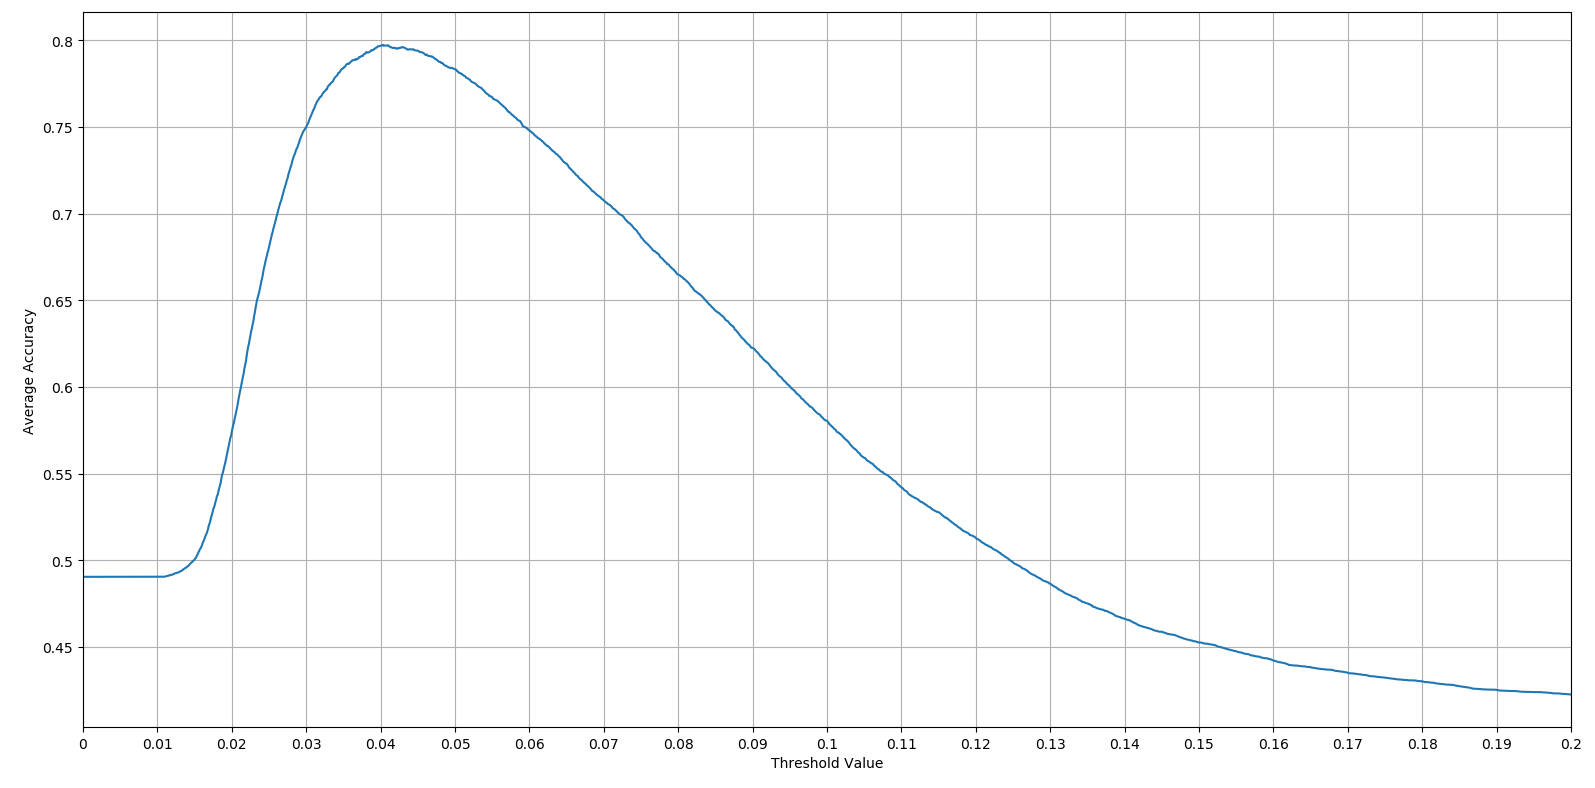
\includegraphics[scale=0.3]{threshold_adjusting.png}
    \caption{Average Accuracy Values for Different Threshold Values (Keypoint Ratio)}
    \label{fig:threshold_new}
  \end{figure}

\begin{table}[H]
    \begin{tabular}{|l|r|r|r|r|r|r|}
        \hline
        \textbf{Test Case}                 & \textbf{TP}   & \textbf{FP} & \textbf{TN} & \textbf{FN} & \textbf{Accuracy} & \textbf{FP Rate} \\ \hline
        Tempo Increase 10\%                & 512         & 13          & 312         & 7           & 0.97630           & 0.04000          \\ \hline
        Tempo Increase 20\%                & 508         & 10          & 315         & 11          & 0.97512           & 0.03077          \\ \hline
        Tempo Increase 50\%                & 501         & 9           & 316         & 18          & 0.96801           & 0.02769          \\ \hline
        Tempo Decrease 10\%                & 515         & 11          & 314         & 4           & 0.98223           & 0.03385          \\ \hline
        Tempo Decrease 20\%                & 519         & 10          & 315         & 0           & 0.98815           & 0.03077          \\ \hline
        Tempo Decrease 50\%                & 519         & 9           & 316         & 0           & 0.98934           & 0.02769          \\ \hline
        Pitch Increase 10\%                & 519         & 9           & 316         & 0           & 0.98934           & 0.02769          \\ \hline
        Pitch Increase 20\%                & 517         & 9           & 316         & 2           & 0.98697           & 0.02769          \\ \hline
        Pitch Increase 50\%                & 0           & 4           & 321         & 519         & 0.38033           & 0.01231          \\ \hline
        Pitch Decrease 10\%                & 516         & 16          & 309         & 3           & 0.97749           & 0.04923          \\ \hline
        Pitch Decrease 20\%                & 503         & 25          & 300         & 16          & 0.95142           & 0.07692          \\ \hline
        Pitch Decrease 50\%                & 23          & 160         & 165         & 496         & 0.22275           & 0.49231          \\ \hline
        Tempo  \& Pitch Increase 10\%      & 413         & 11          & 314         & 106         & 0.86137           & 0.03385          \\ \hline
        Tempo  \& Pitch Increase 20\% & 287         & 17          & 308         & 232         & 0.70498           & 0.05231          \\ \hline
        Tempo  \& Pitch Increase 50\% & 0           & 7           & 318         & 519         & 0.37678           & 0.02154          \\ \hline
        Tempo  \& Pitch Decrease 10\% & 432         & 28          & 297         & 87          & 0.86374           & 0.08615          \\ \hline
        Tempo  \& Pitch Decrease 20\% & 346         & 34          & 291         & 173         & 0.75474           & 0.10462          \\ \hline
        Tempo  \& Pitch Decrease 50\% & 6           & 154         & 171         & 513         & 0.20972           & 0.47385          \\ \hline
    \end{tabular}

\caption{Experiment results using keypoint ratio as threshold}
\label{tab:test_results_keypoint_ratio}
\end{table}
